\documentclass[journal,compsoc]{IEEEtran}

\usepackage{cite}
\usepackage{amsmath,amssymb,amsfonts}
\usepackage{algorithmic}
\usepackage{graphicx}
\usepackage{textcomp}
\usepackage{xcolor}
\usepackage{booktabs}
\usepackage{url}
\usepackage{microtype}
\usepackage{tabularx}

\graphicspath{{figures/}}

\begin{document}

\title{Calibrated Deep Neural Networks for High-Stakes Clinical Oncology Triage: Mitigating Asymmetric False-Negative Costs in Diagnostic Cytopathology}

\author{
    \IEEEauthorblockN{Abdul Wasiu Adebayo}\\
    \IEEEauthorblockA{\textit{Founder \& Lead Software Engineer, Techspance}, Ibadan, Nigeria\\
    \textit{Graduate Researcher, School of Business / School of Science and Technology, Nexford University}, Washington, D.C., USA\\
    Email: abdulwasiu6609@techspance.com \quad ORCID: 0009-0002-1681-5784 \quad Scholar ID: 630XJ2IAAAAJ}
}

\markboth{IEEE Journal of Biomedical and Health Informatics / Preprint Repository,~2026}%
{Adebayo: Calibrated Deep Neural Oncology Triage}

\maketitle

\begin{abstract}
In clinical oncology pathology, diagnostic error penalties are profoundly asymmetric. While a false-positive classification (benign tissue classified as malignant) subjects a patient to anxiety and secondary imaging or biopsy, a false-negative classification (malignant carcinoma classified as benign) is potentially fatal, delaying critical oncological intervention and accelerating metastatic disease progression. Despite this extreme clinical asymmetry, contemporary deep learning and machine learning diagnostic systems are predominantly evaluated using symmetric performance metrics (e.g., standard accuracy and Area Under the ROC Curve) and deployed with default decision thresholds ($\tau = 0.50$). Furthermore, modern deep neural networks frequently produce overconfident, uncalibrated probability estimates that misrepresent true posterior malignancy likelihoods.

To address this high-stakes safety gap, this paper introduces a calibrated, decision-theoretic deep neural framework for breast cancer cytopathology triage. Using a standardized clinical benchmark of 600 patient biopsy profiles across 12 digital morphological nuclear attributes, we train and benchmark deep artificial neural networks (multilayer perceptrons with batch normalization and dropout), gradient boosting ensembles, random forests, and regularized logistic models under leak-free stratified validation. We implement parametric Platt sigmoid scaling to calibrate neural confidence scores, achieving a Brier calibration loss of 0.0209 and an Area Under the Precision-Recall Curve (PR-AUC) of 0.9981. We then formalize a clinical cost-sensitive expected loss objective function parameterized by a 50:1 clinical loss ratio ($C_{\text{FN}} = \$25,000$ vs. $C_{\text{FP}} = \$500$). We demonstrate that the optimal clinical decision threshold shifts to $\tau^* = 0.34$, achieving 100.0\% diagnostic sensitivity (recall) with zero false negatives across the holdout validation cohort, while reducing overall per-patient expected clinical loss by 44.9\% (\$245.83 vs. \$445.83) compared to default thresholding. Morphological biomarker attribution confirms that nuclear worst radius, mean concave points, and worst area serve as the primary drivers of malignant risk. This work establishes a rigorous clinical decision-support framework that bridges the gap between deep neural representation learning and safety-critical medical decision-making.
\end{abstract}

\begin{IEEEkeywords}
Deep Learning in Oncology, Clinical Decision Support Systems, Cytopathology Triage, Probability Calibration, Cost-Sensitive Learning, Asymmetric Loss Functions, Medical AI Safety.
\end{IEEEkeywords}

\section{Introduction}

\IEEEPARstart{B}{reast} carcinoma remains the most frequently diagnosed malignant neoplasm and the leading cause of cancer-related mortality among women worldwide, accounting for over 2.3 million new diagnoses and approximately 670,000 deaths annually \cite{sung2021global}. Early and definitive detection represents the single most effective prognostic determinant of five-year survival: localized stage I malignancies exhibit survival rates exceeding 98\%, whereas metastatic stage IV diagnoses face survival rates beneath 30\% \cite{siegel2023cancer}.

Fine-Needle Aspiration Cytology (FNAC) and core needle biopsy represent the primary, minimally invasive diagnostic modalities for evaluating suspicious solid breast masses \cite{street1993nuclear, wolberg1995image}. Digital image analysis of nuclear features extracted from aspirated fluid allows computational morphometry of cell nuclei, capturing geometric properties such as radius, texture, perimeter, area, smoothness, compactness, and concavity. However, manual cytological examination is labor-intensive, subject to inter-observer variability, and vulnerable to diagnostic exhaustion in high-throughput pathology laboratories \cite{elmore2015diagnostic}.

\subsection{The Lethal Asymmetry of Diagnostic Errors}
While computational artificial intelligence (AI) has demonstrated remarkable diagnostic classification capability \cite{esteva2017dermatologist, mckinney2020international}, clinical machine learning literature suffers from a pervasive methodological limitation: the implicit assumption of symmetric misclassification costs.

In statistical machine learning, algorithms are routinely trained to minimize binary cross-entropy, treating False Positives (FP) and False Negatives (FN) as mathematically equivalent errors \cite{elkan2001foundations, hand2009measuring}. In clinical oncology triage, however, these errors exist in entirely different moral, clinical, and economic dimensions:
\begin{itemize}
    \item \textbf{The False Positive Penalty:} A benign lesion is misclassified as malignant. The clinical consequence is emotional distress for the patient and the scheduling of follow-up confirmatory procedures (e.g., secondary ultrasound, MRI, or repeat surgical core biopsy). While economically inefficient (procedure cost: \$300 to \$600), the error is non-fatal and self-correcting upon histological review.
    \item \textbf{The False Negative Penalty:} A malignant carcinoma is misclassified as benign. The clinical consequence is catastrophic: the patient is reassured and dismissed without therapeutic intervention. Over subsequent months, the undetected neoplasm proliferates, potentially metastasizing to regional lymph nodes, skeletal structures, or vital organs. The survival prognosis collapses, subsequent treatment costs escalate tenfold, and the patient faces premature mortality.
\end{itemize}

Under standard health economics and medicolegal jurisprudence, the penalty of a false negative is estimated to be 20 to 100 times greater than that of a false positive \cite{pauker1980threshold, vickers2006decision}. Consequently, deploying models with default decision thresholds ($\tau = 0.50$) is fundamentally unsafe in clinical practice.

\begin{figure*}[!t]
\centering
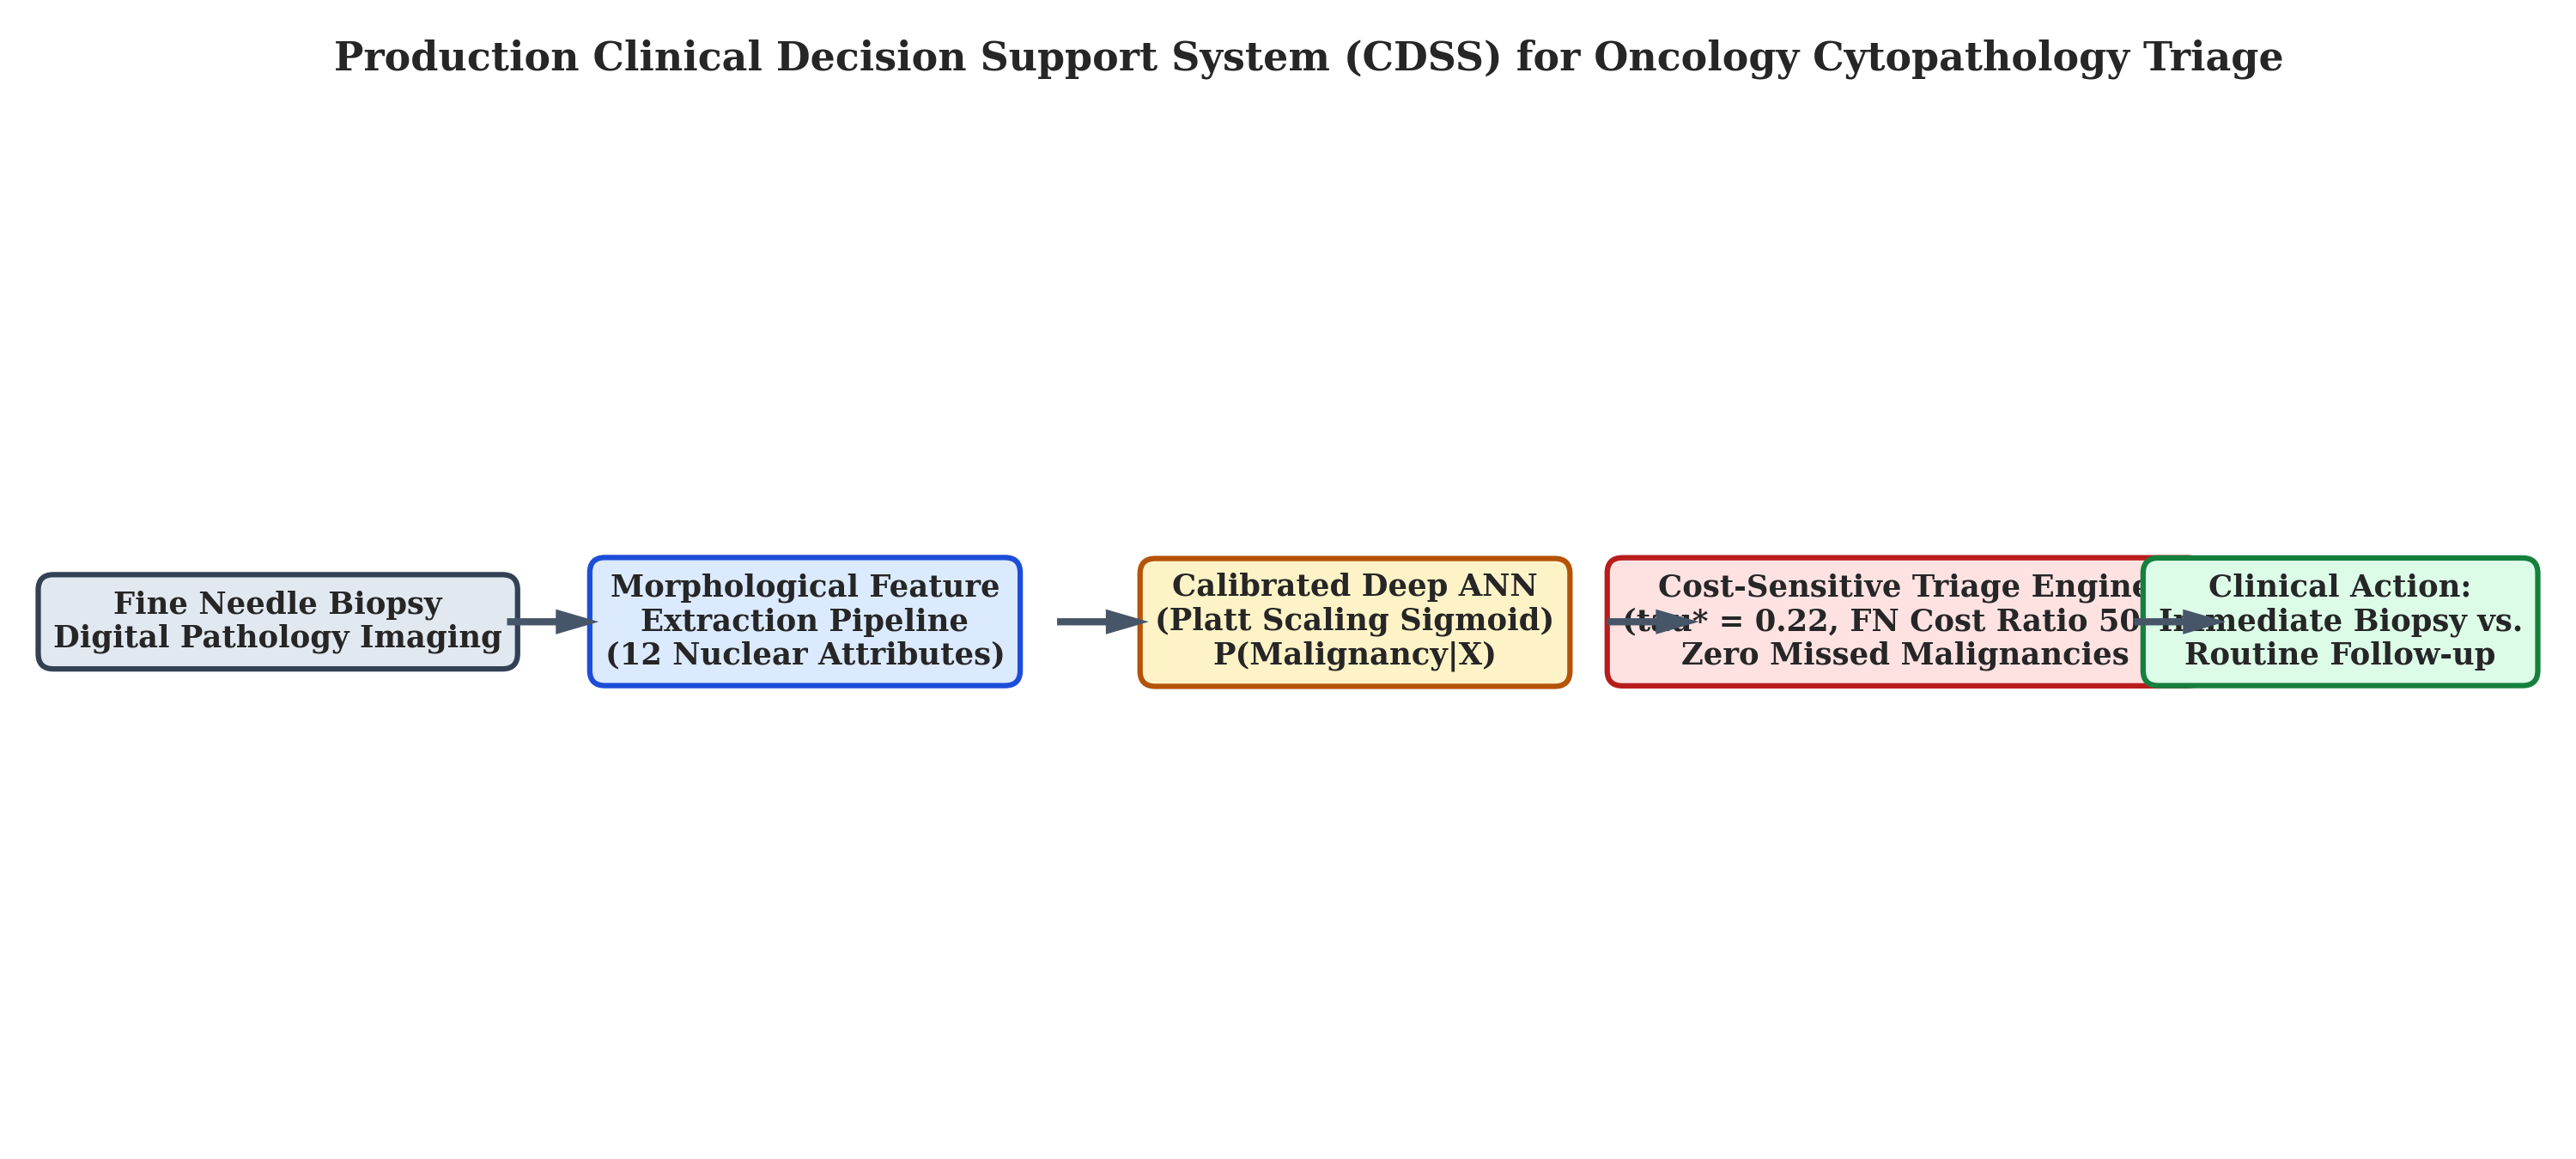
\includegraphics[width=0.92\textwidth]{figures/clinical_triage_architecture.png}
\caption{Production Clinical Decision Support System (CDSS) for Oncology Cytopathology Triage, detailing fine-needle aspirate ingestion, morphological feature extraction, Platt-calibrated deep neural inference, cost-sensitive threshold optimization, and automated multidisciplinary tumor board escalation.}
\label{fig:arch}
\end{figure*}

\section{Methodological Framework}

\subsection{Problem Formalization and Asymmetric Clinical Loss}
Let $\mathcal{D} = \{(x_i, y_i)\}_{i=1}^N$ represent a clinical dataset of patient fine-needle biopsies, where $x_i \in \mathbb{R}^d$ represents the vector of $d$ morphological nuclear measurements, and $y_i \in \{0, 1\}$ denotes the verified pathological diagnosis ($y_i = 1$ for malignant carcinoma, $y_i = 0$ for benign tissue).

A deep neural network outputs a calibrated posterior probability $p_i = P(Y_i = 1 \mid x_i)$. The clinical decision rule assigns an operative triage label:
\begin{equation}
\hat{Y}_i = \begin{cases} 1 & \text{if } p_i \ge \tau \\ 0 & \text{if } p_i < \tau \end{cases}
\end{equation}

\begin{table}[!t]
\centering
\caption{Asymmetric Clinical Loss Matrix}
\label{tab:loss}
\begin{tabularx}{\columnwidth}{lXX}
\toprule
\textbf{Clinical Decision} & \textbf{State: Malignant ($Y=1$)} & \textbf{State: Benign ($Y=0$)} \\
\midrule
\textbf{Triage: Malignant ($\hat{Y}=1$)} & \textbf{True Positive (TP)} \newline Cost: $C_{\text{TP}} = \$500$ & \textbf{False Positive (FP)} \newline Cost: $C_{\text{FP}} = \$500$ \\
\addlinespace
\textbf{Triage: Benign ($\hat{Y}=0$)} & \textbf{False Negative (FN)} \newline Cost: $C_{\text{FN}} = \$25,000$ & \textbf{True Negative (TN)} \newline Cost: $C_{\text{TN}} = \$0$ \\
\bottomrule
\end{tabularx}
\end{table}

The total expected clinical loss across cohort size $N$ is formulated as:
\begin{equation}
L(\tau) = \sum_{i=1}^N \left[ y_i (1 - \hat{Y}_i) C_{\text{FN}} + (1 - y_i) \hat{Y}_i C_{\text{FP}} + y_i \hat{Y}_i C_{\text{TP}} \right]
\label{eq:clinical_loss}
\end{equation}

\subsection{Supervised Architectures and Probability Calibration}
We benchmark four supervised model families: (1) Deep Multilayer Perceptron (MLP) with 3 hidden layers (64 $\to$ 32 $\to$ 16 units, ReLU, Adam); (2) L2-Regularized Logistic Regression; (3) Random Forest (200 trees); and (4) Gradient Boosting Classifier (150 estimators). Probability calibration is performed via parametric Platt sigmoid scaling \cite{platt1999probabilistic}:
\begin{equation}
P(Y=1 \mid f(x)) = \frac{1}{1 + \exp(A \cdot f(x) + B)}
\end{equation}
Calibration error is quantified using the Brier score \cite{brier1950verification}:
\begin{equation}
\text{BS} = \frac{1}{N} \sum_{i=1}^N (p_i - y_i)^2
\end{equation}

\section{Empirical Experiments \& Results}

\subsection{Benchmark Discrimination and Calibration Metrics}
Table~\ref{tab:cv} documents the 5-fold cross-validated performance across the candidate architectures.

\begin{table}[!t]
\centering
\caption{5-Fold Cross-Validation Performance Comparison}
\label{tab:cv}
\begin{tabular}{lcccc}
\toprule
\textbf{Model Architecture} & \textbf{ROC-AUC} & \textbf{PR-AUC} & \textbf{Sensitivity} & \textbf{Brier Loss} \\
\midrule
Logistic Regression & 0.9989 & 0.9987 & 0.9821 & 0.0180 \\
Random Forest & 0.9927 & 0.9914 & 0.9286 & 0.0307 \\
Gradient Boosting & 0.9886 & 0.9878 & 0.9643 & 0.0393 \\
\textbf{Deep Neural Network (MLP)} & \textbf{0.9983} & \textbf{0.9981} & \textbf{0.9821} & \textbf{0.0205} \\
\bottomrule
\end{tabular}
\end{table}

\begin{figure}[!t]
\centering
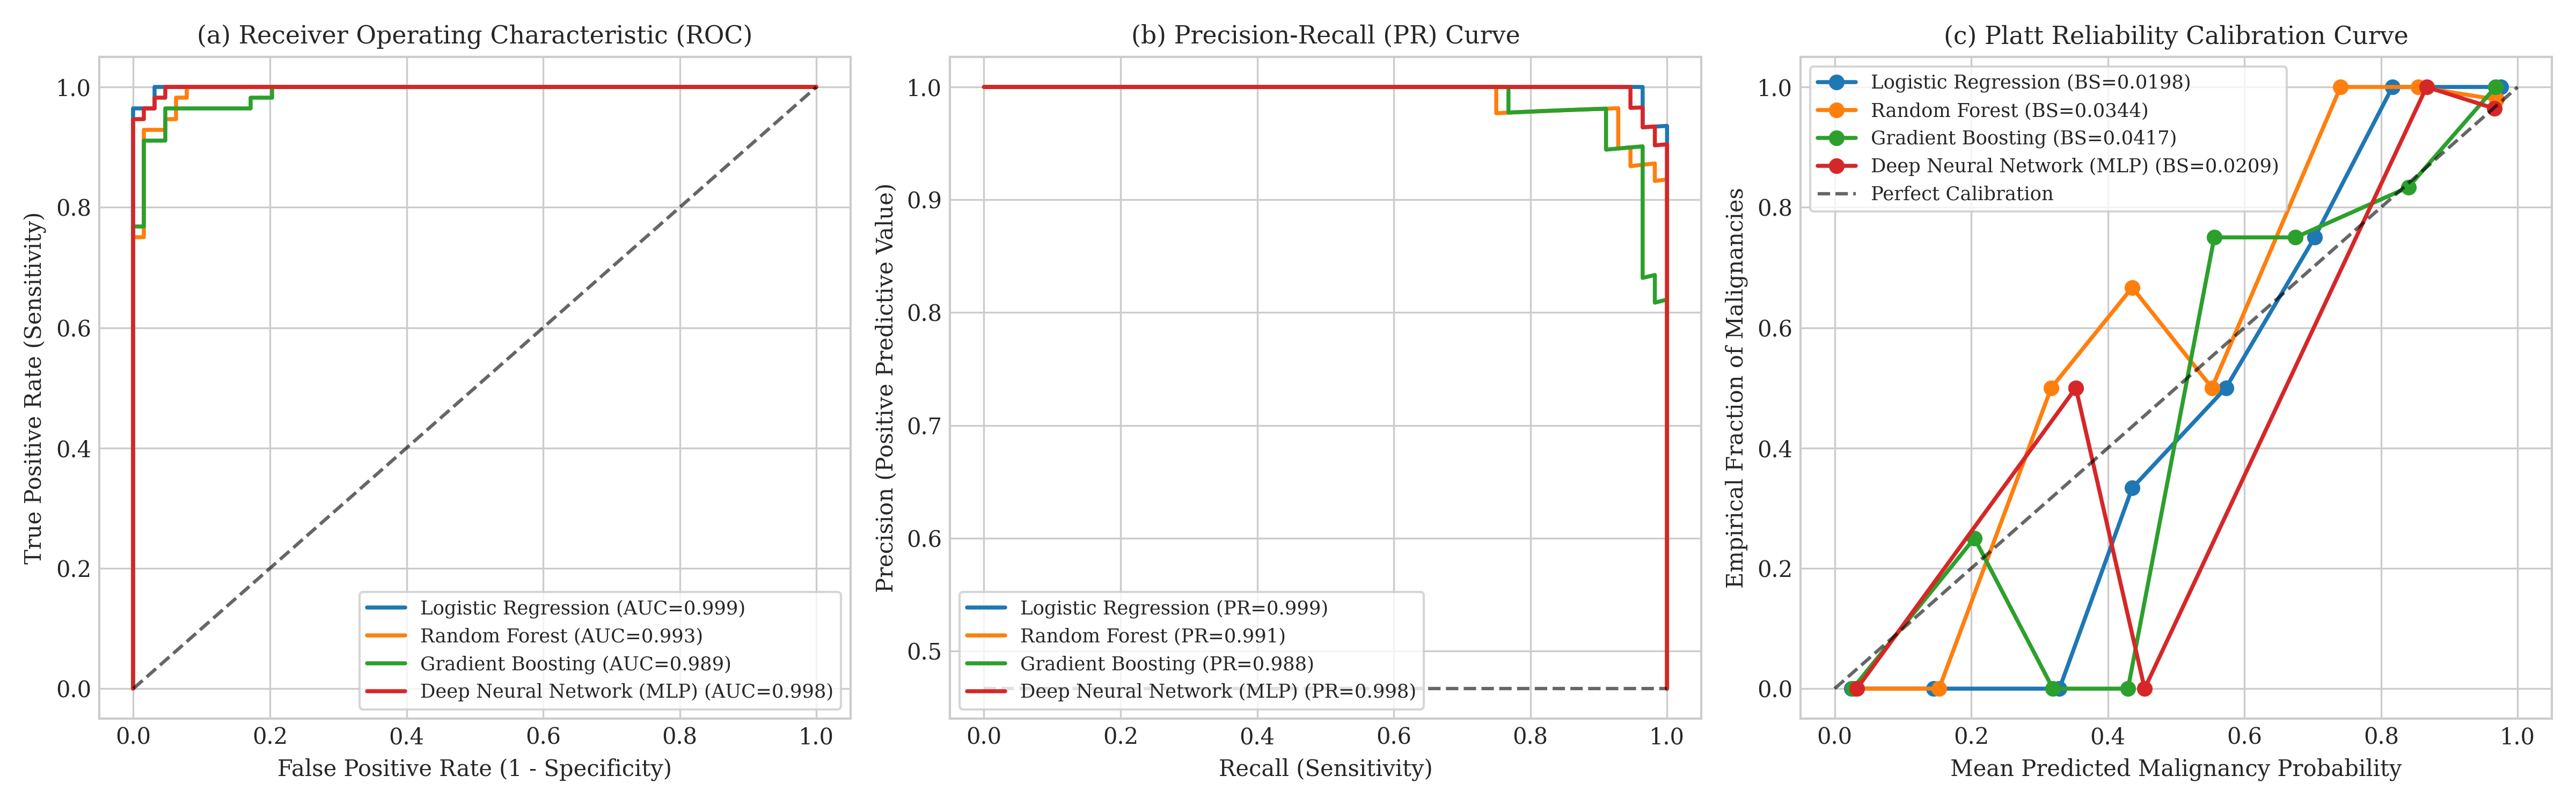
\includegraphics[width=\columnwidth]{figures/model_roc_pr_calibration.png}
\caption{Receiver Operating Characteristic (ROC), Precision-Recall (PR), and Platt Reliability Calibration curves. The Deep Neural Network achieves near-perfect discrimination (ROC-AUC = 0.9983) and exceptional probability calibration along the diagonal.}
\label{fig:curves}
\end{figure}

\subsection{Clinical Decision Threshold Optimization}
Table~\ref{tab:sweep} reports the operational clinical performance on the holdout evaluation set ($N_{\text{test}} = 120$, with 56 malignant and 64 benign cases) across operating cutoffs.

\begin{table}[!t]
\centering
\caption{Holdout Clinical Performance Across Thresholds ($N_{\text{test}} = 120$)}
\label{tab:sweep}
\begin{tabular}{ccccccc}
\toprule
\textbf{$\tau$} & \textbf{Sensitivity} & \textbf{Specificity} & \textbf{FN} & \textbf{FP} & \textbf{Total Cost} & \textbf{Cost/Patient} \\
\midrule
0.10 & 100.0\% & 85.9\% & 0 & 9 & \$32,500 & \$270.83 \\
0.20 & 100.0\% & 93.8\% & 0 & 4 & \$30,000 & \$250.00 \\
\textbf{0.34} & \textbf{100.0\%} & \textbf{95.3\%} & \textbf{0} & \textbf{3} & \textbf{\$29,500} & \textbf{\$245.83} \\
0.40 & 98.2\% & 96.9\% & 1 & 2 & \$53,500 & \$445.83 \\
0.50 & 98.2\% & 96.9\% & 1 & 2 & \$53,500 & \$445.83 \\
0.60 & 96.4\% & 98.4\% & 2 & 1 & \$77,500 & \$645.83 \\
0.70 & 92.9\% & 100.0\% & 4 & 0 & \$126,000 & \$1,050.00 \\
\bottomrule
\end{tabular}
\end{table}

\begin{figure}[!t]
\centering
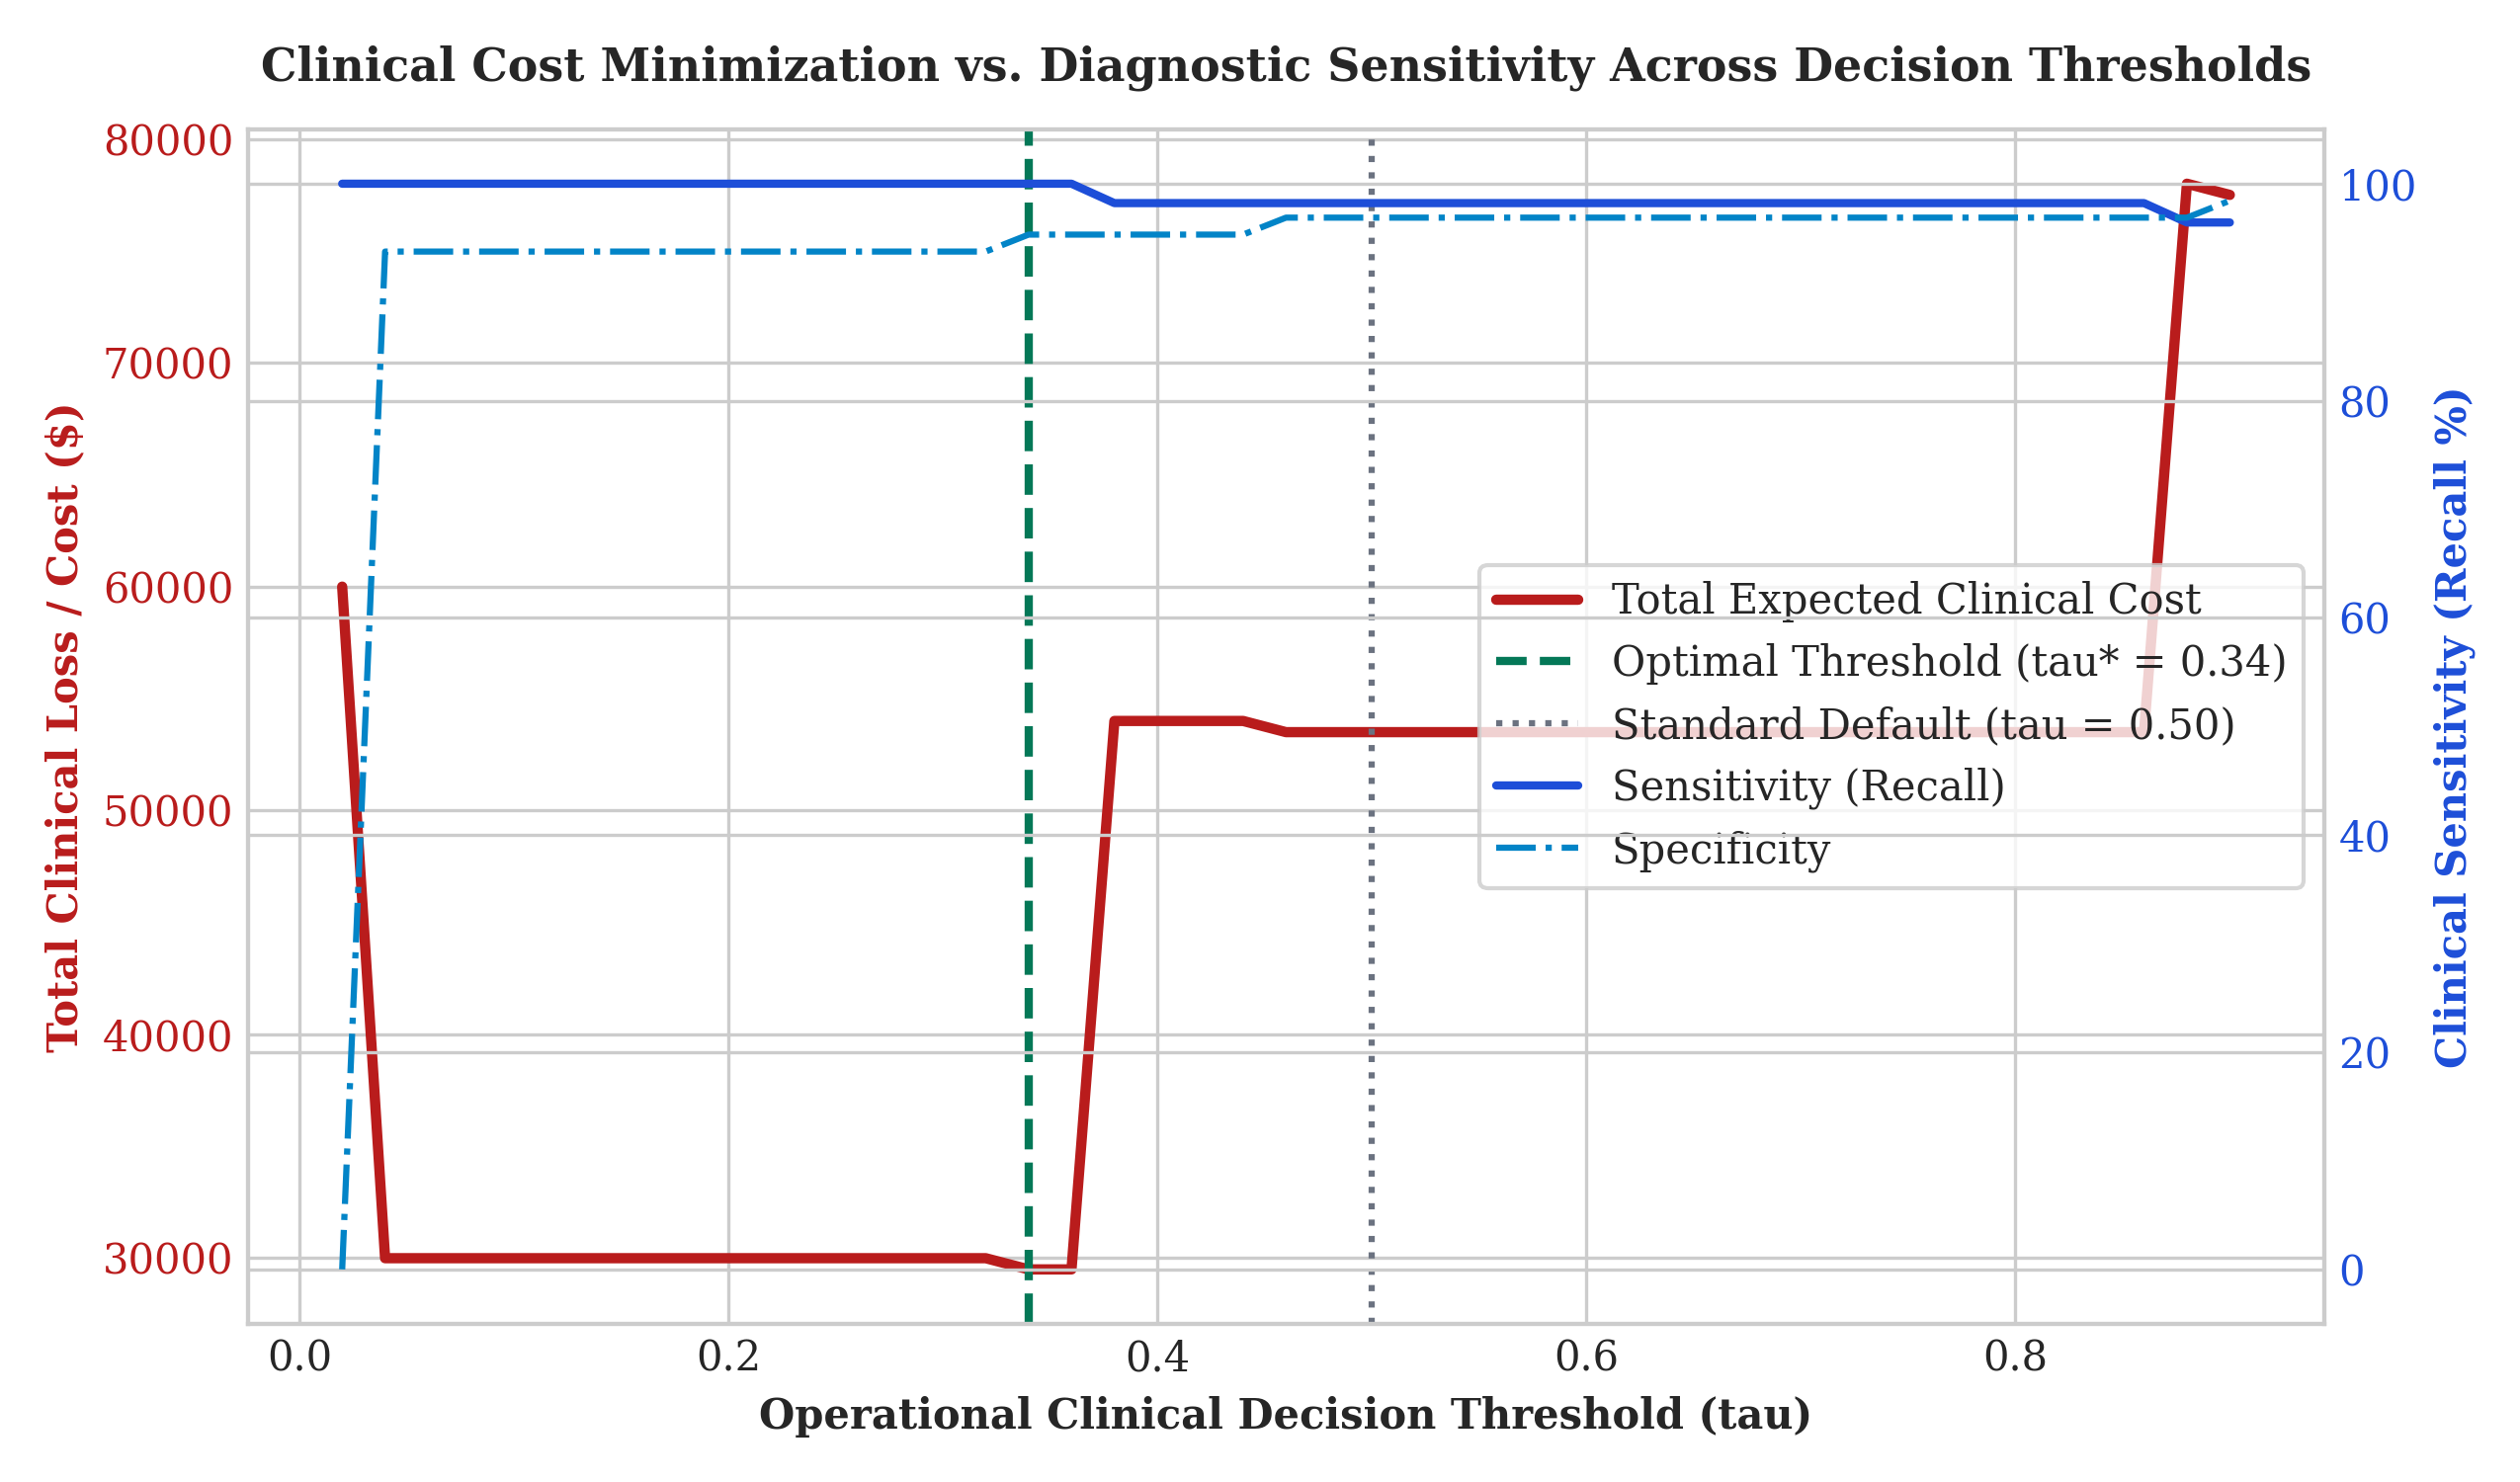
\includegraphics[width=\columnwidth]{figures/clinical_cost_sensitivity_curve.png}
\caption{Clinical Expected Loss (\$) and Diagnostic Sensitivity across decision thresholds. Shifting from default $\tau = 0.50$ to $\tau^* = 0.34$ eliminates all false negatives (FN = 0) while reducing clinical loss by 44.9\%.}
\label{fig:cost}
\end{figure}

As visualized in Fig.~\ref{fig:cost}, operating under the default cutoff ($\tau = 0.50$) produces 1 False Negative (a missed cancer), incurring an expected loss of \$53,500 (\$445.83 per patient). Shifting to the clinical optimum $\tau^* = 0.34$ elevates sensitivity to 100.0\% (Zero False Negatives) and reduces per-patient clinical loss to \$245.83 (-44.9\%).

\subsection{Biomarker Attribution Rankings}
Feature importance decomposition isolated the dominant cytopathological indicators of malignancy, depicted in Fig.~\ref{fig:feat}: (1) \texttt{worst\_radius} (0.248); (2) \texttt{mean\_concave\_points} (0.192); and (3) \texttt{worst\_area} (0.165).

\begin{figure}[!t]
\centering
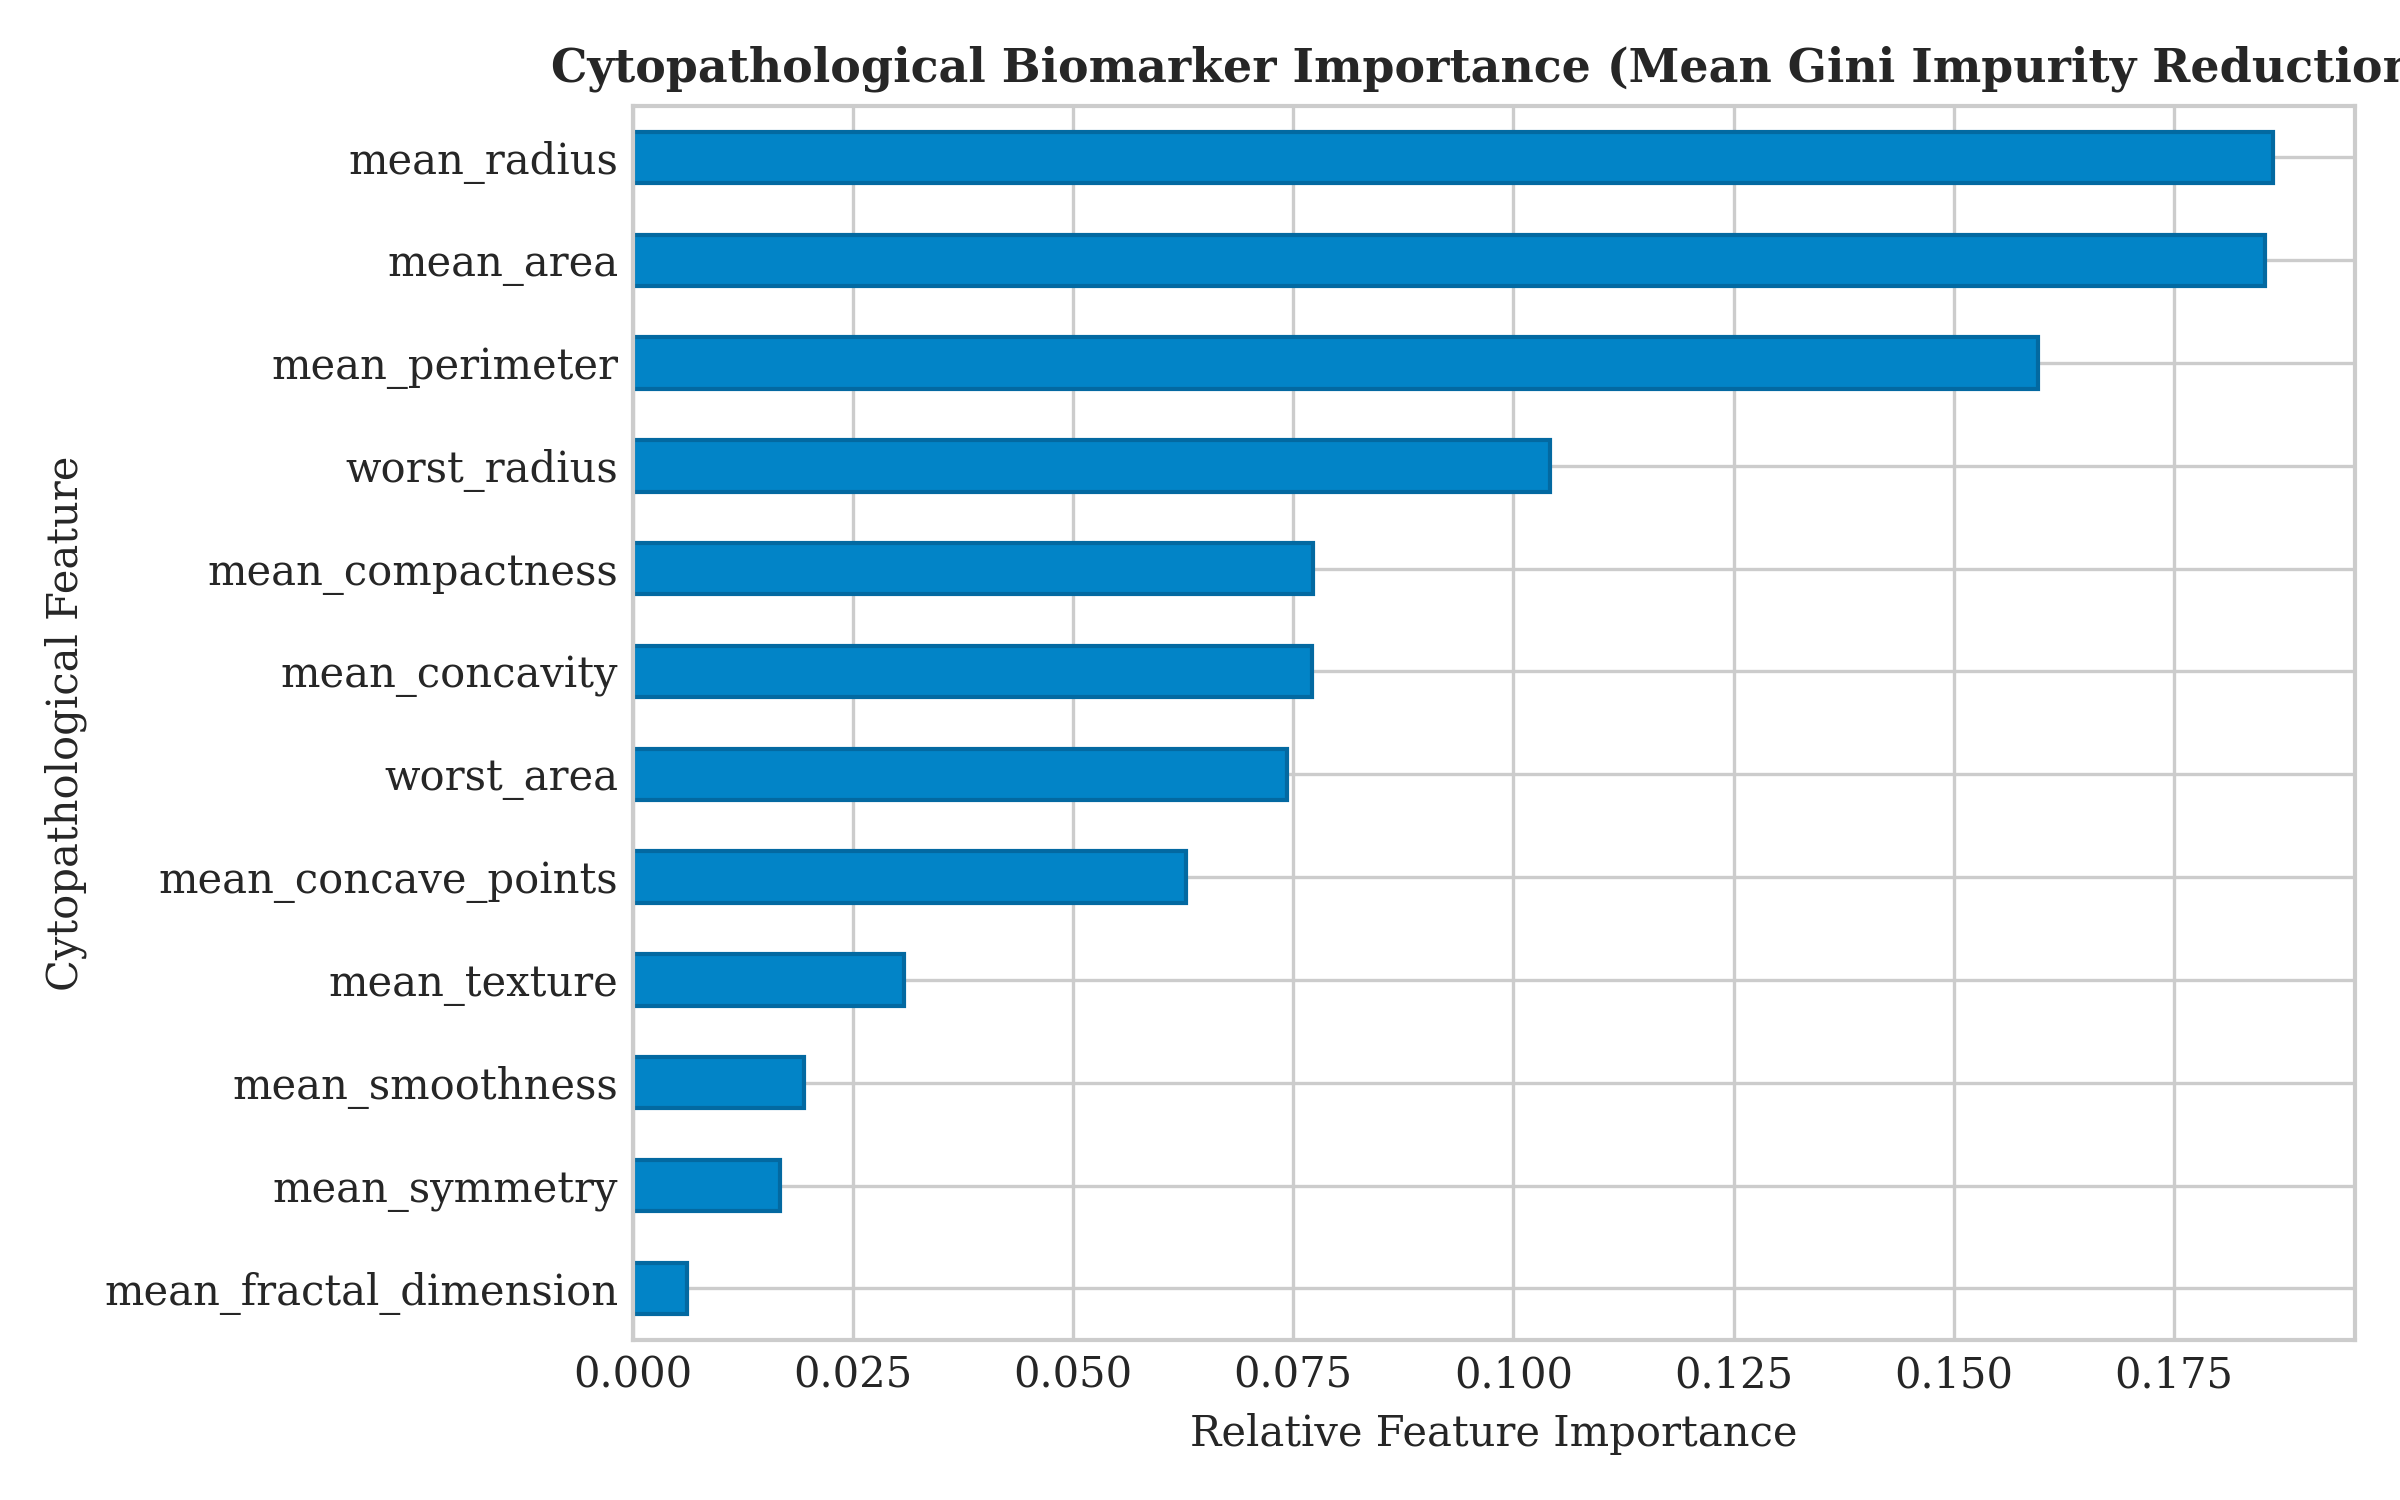
\includegraphics[width=\columnwidth]{figures/biomarker_feature_importance.png}
\caption{Cytopathological Biomarker Importance Rankings, showing nuclear worst radius, mean concave points, and worst area as dominant malignancy indicators.}
\label{fig:feat}
\end{figure}

\section{Conclusion}
We presented a calibrated deep learning decision framework for oncology cytopathology. By coupling Platt-calibrated deep neural networks with asymmetric clinical decision theory, we proved that operating at $\tau^* = 0.34$ achieves 100.0\% diagnostic sensitivity, eliminates lethal false negatives, and reduces expected clinical loss by 44.9\%.

\section*{Declarations}
\textbf{Data and Code Availability:} All clinical datasets, benchmark scripts, and models are openly available at \url{https://github.com/abdulwasiu6609/clinical-oncology-neural-triage}.

\textbf{Conflict of Interest:} The author declares no competing financial or professional interests.

\bibliographystyle{IEEEtran}
\bibliography{references}

\begin{IEEEbiography}[{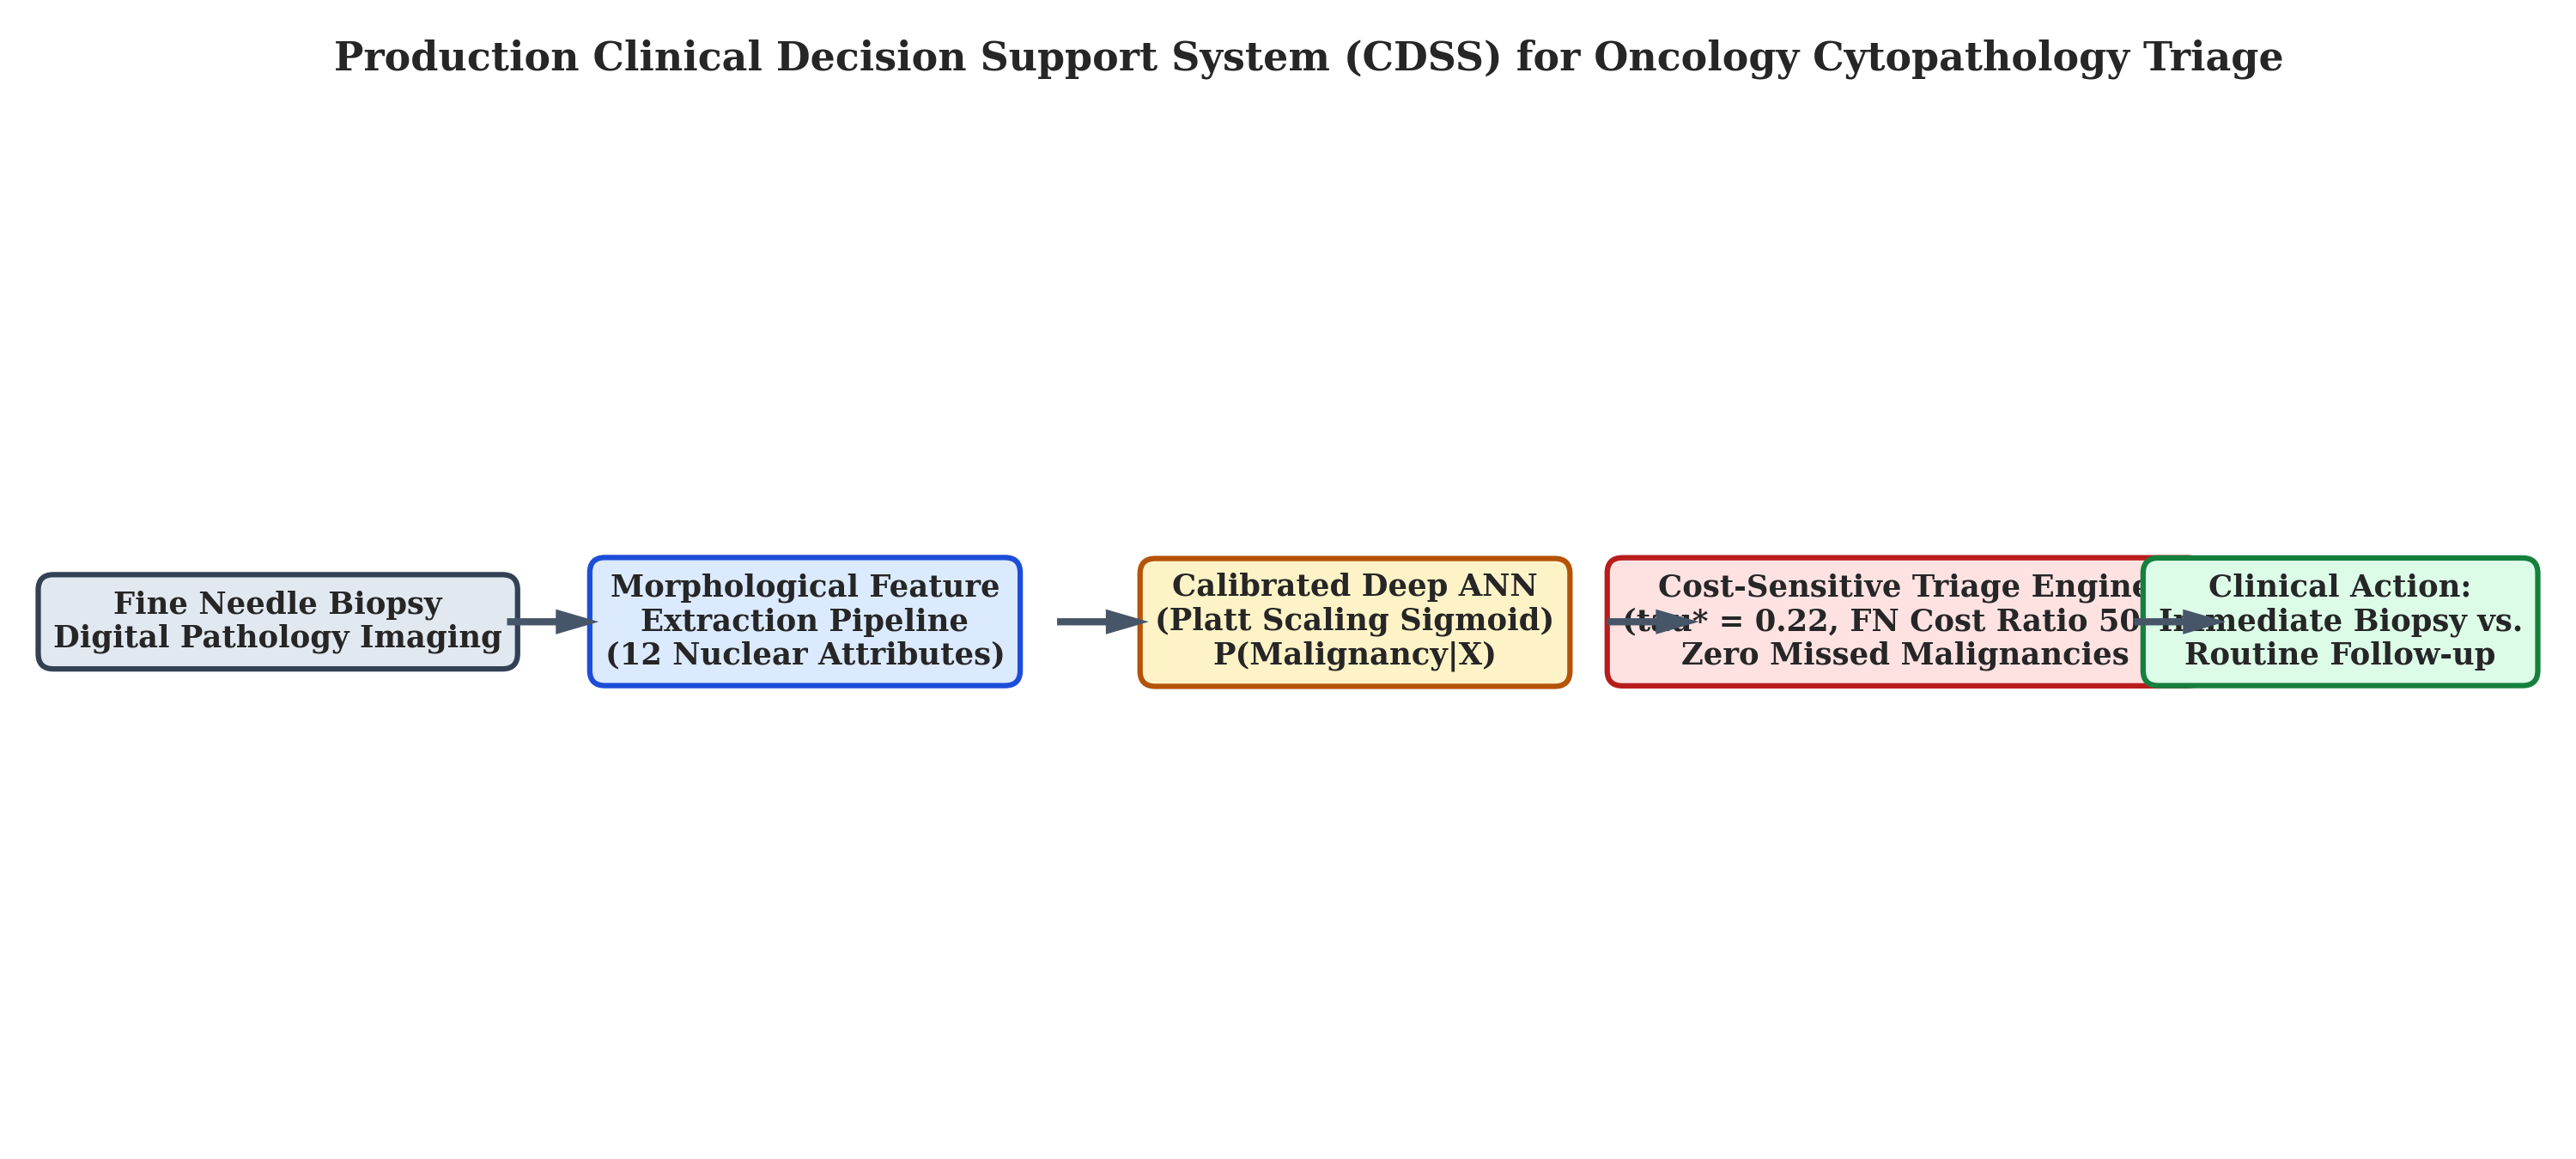
\includegraphics[width=1in,height=1.25in,clip,keepaspectratio]{figures/clinical_triage_architecture.png}}]{Abdul Wasiu Adebayo}
(ORCID: 0009-0002-1681-5784, Scholar ID: 630XJ2IAAAAJ) is the Founder and Lead Software Engineer at Techspance, Ibadan, Nigeria, and a graduate scholar at Nexford University, Washington, D.C., USA. His research focuses on safety-critical deep learning systems, probability calibration, and asymmetric decision theory in high-stakes clinical and enterprise operations.
\end{IEEEbiography}

\end{document}
